\begin{table}[ht!]
	\centering
		\begin{tabular}{c |c| c |c| c|c}
			
			\toprule
			& CV-H& CV-L& VCV-LH& CVV-LH& CVV-HL\\
			\midrule
			
			\textbf{UR}
			
			&
			
			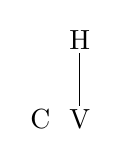
\begin{tikzpicture}[scale=1, every node/.style={inner sep=1pt}]
				\node (c1) at (-.5,0) {C};
				\node (v1) at (0,0) {V};
				\node (t1) at (0,1) {H};
				\draw (v1)--(t1);
			\end{tikzpicture}
			
			&
			
			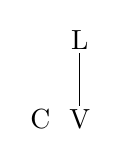
\begin{tikzpicture}[scale=1, every node/.style={inner sep=1pt}]
				\node (c1) at (-.5,0) {C};
				\node (v1) at (0,0) {V};
				\node (t1) at (0,1) {L};
				\draw (v1)--(t1);
			\end{tikzpicture}
			
			&
			
			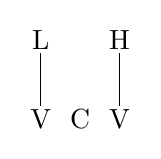
\begin{tikzpicture}[scale=1, every node/.style={inner sep=1pt}]
%				\node (c1) at (-.5,0) {C};
				\node (v1) at (0,0) {V};
				\node (c2) at (.5,0) {C};
				\node (t1) at (0,1) {L};
				\node (v2) at (1,0) {V};
				\node (t2) at (1,1) {H};
				\draw (v1)--(t1);
				\draw (v2)--(t2);
			\end{tikzpicture}
			
			&
			
			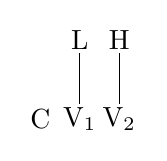
\begin{tikzpicture}[scale=1, every node/.style={inner sep=1pt}]
				\node (c1) at (-.5,0) {C};
				\node (v1) at (0,0) {V$_1$};
				\node (t1) at (0,1) {L};
				\node (v2) at (.5,0) {V$_2$};
				\node (t2) at (.5,1) {H};
				\draw (v1)--(t1);
				\draw (v2)--(t2);
			\end{tikzpicture}
						&
			
			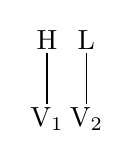
\begin{tikzpicture}[scale=1, every node/.style={inner sep=1pt}]
%				\node (c1) at (-.5,0) {C};
				\node (v1) at (0,0) {V$_1$};
				\node (t1) at (0,1) {H};
				\node (v2) at (.5,0) {V$_2$};
				\node (t2) at (.5,1) {L};
				\draw (v1)--(t1);
				\draw (v2)--(t2);
			\end{tikzpicture}
			\\
			
			\midrule
			
			\textbf{SR}
			
			& -- & -- & --
			
			&
			
			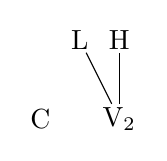
\begin{tikzpicture}[scale=1, every node/.style={inner sep=1pt}]
				\node (c1) at (-.5,0) {C};
				\node (t1) at (0,1) {L};
				\node (v2) at (.5,0) {V$_2$};
				\node (t2) at (.5,1) {H};
				\draw (v2)--(t1);
				\draw (v2)--(t2);
			\end{tikzpicture}
			&

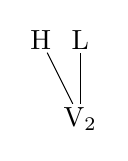
\begin{tikzpicture}[scale=1, every node/.style={inner sep=1pt}]
%	\node (c1) at (-.5,0) {C};
	\node (t1) at (0,1) {H};
				\node (v2) at (.5,0) {V$_2$};
	\node (t2) at (.5,1) {L};
	\draw (v2)--(t1);
	\draw (v2)--(t2);
\end{tikzpicture}			
			\\
			
			\bottomrule
			
		\end{tabular}
	
		
\caption{Toy ASG}
\label{tab.toy}
\end{table}